% \documentclass{article}
% \usepackage{arxiv}

% \usepackage[utf8]{inputenc}
% \usepackage[english, russian]{babel}
% \usepackage[T1]{fontenc}
% \usepackage{url}
% \usepackage{booktabs}
% \usepackage{amsfonts}
% \usepackage{nicefrac}
% \usepackage{microtype}
% \usepackage{lipsum}
% \usepackage{graphicx}
% \usepackage{natbib}
% \usepackage{doi}
% \usepackage{amsmath}
% \usepackage{hyperref}
% \usepackage{caption}
% \DeclareMathOperator*{\argmax}{arg\,max}
% \DeclareMathOperator*{\argmin}{arg\,min}
\documentclass[a4paper,12pt]{article}

\usepackage[T2A]{fontenc}
\usepackage[utf8]{inputenc}
\usepackage[english,russian]{babel}
\usepackage{tikz}                % для создания иллюстраций
\usepackage{pgfplots}            % для вывода графиков функций
\usepackage{geometry}		 % для настройки размера полей
\usepackage{indentfirst}         % для отступа в первом абзаце секции
\def\code#1{\texttt{#1}}
\usepackage{float}

% выбираем размер листа А4, все поля ставим по 3см
\geometry{a4paper,left=30mm,top=30mm,bottom=30mm,right=30mm}

\setcounter{secnumdepth}{0}      % отключаем нумерацию секций

\usepgfplotslibrary{fillbetween} % для изображения областей на графиках
%\usepackage{graphics}
\usepackage{graphicx}
\usepackage{amsmath}
\usepackage{amsthm}
\usepackage{wasysym}
\usepackage{amssymb}
\usepackage{hyperref}
\usepackage{url}
\usepackage{booktabs}
\usepackage{amsfonts}
\usepackage{nicefrac}
\usepackage{microtype}
\usepackage{natbib}
\usepackage{doi}
\usepackage{caption}
\DeclareMathOperator*{\argmax}{arg\,max}
\DeclareMathOperator*{\argmin}{arg\,min}
\linespread{1.5}
\hypersetup{
    colorlinks=true,
    linkcolor=black,
    filecolor=magenta,      
    urlcolor=blue
    }

\title{Выпускная квалификационная работа}

\author{ Валентин А. Абрамов \\
	Факультет вычислительной математики и кибернетики\\
	МГУ имени М. В. Ломоносова\\
	%% \AND
	%% Coauthor \\
	%% Affiliation \\
	%% Address \\
	%% \texttt{email} \\
	%% \And
	%% Coauthor \\
	%% Affiliation \\
	%% Address \\
	%% \texttt{email} \\
	%% \And
	%% Coauthor \\
	%% Affiliation \\
	%% Address \\
	%% \texttt{email} \\
}
\date{}

% \renewcommand{\shorttitle}{\textit{arXiv} Template}
% \renewcommand{\abstractname}{Аннотация}
%%% Add PDF metadata to help others organize their library
%%% Once the PDF is generated, you can check the metadata with
%%% $ pdfinfo template.pdf
% \hypersetup{
% pdftitle={A template for the arxiv style},
% pdfsubject={q-bio.NC, q-bio.QM},
% pdfauthor={David S.~Hippocampus, Elias D.~Striatum},
% pdfkeywords={First keyword, Second keyword, More},
% }

\begin{document}

\begin{titlepage}
\begin{center}
    Московский государственный университет имени М. В. Ломоносова

    \bigskip
    
\includegraphics[width=50mm]{msu.eps}

    \bigskip
    Факультет Вычислительной Математики и Кибернетики\\
    Кафедра Математических Методов Прогнозирования\\[10mm]

    \textsf{\large\bfseries
         Выпускная квалификационная работа\\[10mm]
        <<Эволюционный алгоритм подбора гиперпараметров моделей>>
    }\\[10mm]

    \begin{flushright}
        \parbox{0.5\textwidth}{
            Выполнил:\\
            студент 4 курса 417 группы\\
            \emph{Абрамов Валентин Андреевич}\\[5mm]
            Научный руководитель:\\
            к.ф.-м.н.\\
            \emph{Китов Виктор Владимирович}
        }
    \end{flushright}

    \vspace{\fill}
    Москва
    
    2024
\end{center}
\end{titlepage}
% Автоматически генерируем оглавление на отдельной странице
\tableofcontents
\newpage

\section{Введение}

В последние годы машинное обучение стало одной из самых активно 
развивающихся областей в информационных технологиях. Чтобы достичь 
оптимального качества моделей машинного обучения, необходимо правильно 
настроить конфигурацию этих моделей, то есть тщательно подобрать 
наилучшие гиперпараметры для этих моделей.
Примерами гиперпараметров выступает число K в методе K ближайших 
соседей, сила регуляризации в линейных моделях, число слоев и нейронов на 
каждом слое в нейронных сетях и т.д.

Гиперпараметры являются важными параметрами моделей машинного 
обучения, которые не могут быть настроены по обучающей выборке 
градиентными методами — для этого необходимо оценивать точность модели 
на отдельной валидационной выборке либо перебирая всевозможные 
гиперпараметры вручную (что требует экспертизы и занимает много времени), 
либо используя автоматические методы безградиентной оптимизации. 
Простейшие методы автоматического выбора гиперпараметров, такие как 
перебор по равномерной сетке или случайный поиск, могут быть 
неэффективными или требовать значительных вычислительных ресурсов, 
поэтому вместо них используют более сложные алгоритмы, например, 
эволюционные.  Одним из таких алгоритмов является метод DEHB.


\section{Обзор литературы}

Гиперпараметрическая оптимизация — большая и перспективная область исследований. В данный момент в исследованиях поднимаются вопросы переобучения гиперпараметров на валидационную выборку и параллелизации алгоритмов. Для глубоких нейронных сетей также необходимо подбирать гиперпараметры, такие как число слоев, скорость обучения и даже связи между слоями.
Задача автоматического подбора гиперпараметров активно исследуется. Широко используемые методы перебора значений по сетке и случайного поиска имеют низкую вычислительную эффективность, поскольку не учитывают информацию о качестве ранее протестированных конфигураций (наборов гиперпараметров) для генерации новых конфигураций. В 2011 году был создан подход SMBO — последовательная оптимизация, основанная на суррогатной функции, то есть функции, приближающей целевую оптимизируемую функцию, но быструю для расчета. В качестве суррогатной функции изначально брали гауссовские процессы, но они подходят не для всех задач, так как предназначены только для непрерывных гиперпараметров. 
На данный момент одним из лучших методов автоматического подбора гиперпараметров является метод TPE, основанный на байесовском подходе. Также существуют методы, основанные на подходе SMBO, такие как SMAC, использующий случайный лес в качестве суррогата, или модели, использующие суррогат на основе гауссовских процессов. Также стоит упомянуть об эволюционных алгоритмах, так как они позволяют оптимизировать любые функции за счет интеллектуального перебора значений, основанного на таких идеях эволюции, как мутация, скрещивание, селекция и естественный отбор. Хорошее качество обеспечивает метод Successive Halving (SH)  – он позволяет найти лучший набор гиперпараметров в условиях ограниченности вычислительных мощностей. На основе SH созданы алгоритмы HyperBand, автоматически выделяющий ресурсы для нескольких запусков SH, BOHB, добавляющий в HyperBand суррогат на основе подходов TPE, и DEHB, добавляющий в HyperBand идею дифференциальной эволюции.

\section{Постановка задачи}
Задача гиперпараметрической оптимизации состоит в том, чтобы имея набор данных $X \in \mathbb{R}^{N\times d}, y \in \mathbb{R}^{N}$, пространство гиперпараметров $\Theta \in \mathbb{R}^k$, модель $f(\theta): \mathbb{R}^{d} \to \mathbb{R},\ \theta \in \Theta$, $f \in \mathbb{H}$ и функцию ошибок $\mathcal{L}(f, X, y): \mathbb{H} \times \mathbb{R}^{N\times d} \times \mathbb{R}^{N} \to \mathbb{R}$, найти $\theta^*$ такую, что выполнено
$$\theta^* = \argmin_{\theta} \mathcal{L}(f(\theta), X, y)$$
Таким образом, зная модель $f$, пространство гиперпараметров $\Theta$, набор данных $X, y$ и функцию ошибок $\mathcal{L}$, необходимо найти набор гиперпараметров $\theta^*$, при котором значение функции ошибок $\mathcal{L}$ наименьшее при обучении модели $f$ на данных $X, y$.

Предполагается, что набор гиперпараметров состоит из непрерывных и категориальных переменных, функция $\mathcal{L}$ имеет бюджет вычислений. Им может быть ограничение на максимальное число итераций при обучении нейронной сети, количество деревьев в случайном лесе и градиентном бустинге и т. п.


\section{Существующие методы}
\subsection{Поиск по сетке}
Поиск по сетке работает следующим образом:
\begin{enumerate}
    \item Задаются наборы значений параметров.
    \item Для каждой комбинации параметров вычисляется значение целевой функции.
\end{enumerate}

У этого подхода есть множество известных проблем:
\begin{enumerate}
    \item Необходимость выбора сетки значений вручную.
    \item Медленное время работы.
    \item Многократное вычисление целевой функции при одном и том же значении каждого параметра.
\end{enumerate}


\subsection{Случайный поиск}
Случайный поиск работает следующим образом:
\begin{enumerate}
    \item Наборы параметров случайно сэмплируются из некоторого распределения.
    \item Для каждого набора параметров вычисляется значение целевой функции.
\end{enumerate}

Случайный поиск избавлен от проблем поиска по сетке, но при этом полностью полагается на случайность.

\subsection{Эволюционный алгоритм}
Классический эволюционный алгоритм работает следующим образом:
\begin{enumerate}
    \item Создается набор кандидатов размера $N$, называемый популяцией.
    \item Повторяются следующие действия:
    \begin{enumerate}
        \item Вычисляется значение оптимизируемой функции для каждого кандидата.
        \item Отбирается $M$ лучших по значению функции кандидатов.
        \item Создаются новые $N - M$ кандидатов путём скрещивания $2$ случайных кандидатов из $M$ лучших и мутации.
    \end{enumerate}
\end{enumerate}

Начальные кандидаты сэмплируются из равномерного распределения.
В качестве операции скрещивания используется биномиальное скрещивание -- выбор значения параметра одного из кандидатов-родителей с вероятностью $0.5$. Мутация -- замена параметра на случайное значение с шансом $p$. В таком подходе $N, p$ -- параметры эволюционного алгоритма, эволюция происходит пока не будет достигнуто определенное число итераций или время работы или пока лучшее достигнутое значение оптимизируемой функции не перестанет изменяться в течение некоторого заранее определенного числа итераций. Результат работы такого алгоритма - лучший кандидат по значению функции. 

Перечислим слабые стороны эволюционных алгоритмов:
\begin{enumerate}
    \item Алгоритмы требуют многократного вычисления функции $f$, которая может вычисляться очень долго при обучении моделей.
    \item При мутации не учитывается положительный опыт, есть риск ухудшения набора гиперпараметров при неудачном сэмплировании.
\end{enumerate}

\subsection{Successive Halving}
Successive Halving -- алгоритм подбора гиперпараметров, подразумевающий наличие бюджета вычислений, то есть целевую функцию $f$ можно вычислить с фиксированным бюджетом. Например, можно ограничить количество итераций вычисления $f$ для некоторого численного метода или ограничить число деревьев при обучении случайного леса. 
У алгоритма есть три гиперпараметра: количество начальных кандидатов $N$, минимальный бюджет $\lambda$ и $\eta$ -- параметр шкалирования. На первой итерации из равномерного распределения сэмплируются $N_1$ кандидатов, для них вычисляется функция $f$ с бюджетом $\lambda_1$. На второй итерации берутся $N_2 = N_1/\eta$ лучших кандидатов, для них вычисляется $f$ с бюджетом $\lambda_2 = \eta\lambda_1$. На i-ой итерации функция $f$ вычисляется для $N_i = N_1/\eta^{i - 1}$ лучших кандидатов с шага $i - 1$ с бюджетом $\lambda_i = \eta^{i - 1}\lambda_1$. $\lambda_1$ и $N_1$ выбираются так, что итоговый бюджет вычислений и количество кандидатов составляет $N\lambda$.  Таким образом, алгоритм работает как случайный поиск, который выделяет больше ресурсов перспективным кандидатам и отсекает тех, кто при низком бюджете показывает себя хуже остальных.

\subsection{HyperBand}
HyperBand расширяет идеи SH -- производится несколько запусков SH с различными значениями $N$ и $\lambda$. Для каждого нового запуска уменьшается число кандидатов и увеличивается минимальный бюджет. Таким образом, функции $f$, которые долго сходятся, проверяются для случайных инициализаций и с низким бюджетом, и с высоким. 
У SH и HyperBand есть следующие слабые стороны:
\begin{enumerate}
    \item Алгоритмы полностью полагаются на случайное сэмплирование.
    \item Алгоритмы не генерируют новых кандидатов, учитывая положительный опыт.
    \item Не всегда гиперпараметры, отсеянные при низком бюджете, являются плохими при высоком.
\end{enumerate}

\subsection{Tree-structured Parzen estimator}
Данный метод в начале работает как случайный поиск, а после оценки некоторого заранее заданного числа значений функции начинает действовать по следующему алгоритму:
\begin{enumerate}
    \item Набор параметров строится следующим образом. Для каждого параметра выполняются действия:
    \begin{enumerate}
        \item На основе значений целевой функции строятся распределения $l_{par}(x)$ лучших значений параметра и $g_{par}(x)$ худших значений параметра.
        \item Сэпмлируются новые значения параметра из $l_{par}(x)$.
        \item Выбирается значение параметра с максимальным значением Expected Improvement: $EI = \frac{l_{par}(x)}{g_{par}(x)}$
    \end{enumerate}
    \item Для полученного набора параметров вычисляется значение целевой функции.
    
\end{enumerate}

Данный алгоритм является одним из самых технически продвинутых на данный момент, но у него также есть слабые стороны:
\begin{enumerate}
    \item Для корректного построения распределений параметров $l_{par}(x)$ и $g_{par}(x)$ необходим ``прогрев'' случайным поиском в течение большого числа итераций.
    \item Алгоритм требует многократного вычисления функции $f$, которая может вычисляться очень долго при обучении моделей.
\end{enumerate}

Стоит сказать, что есть и другие методы, например, основанные на байесовской оптимизации, но они работают только с непрерывными гиперпараметрами, а на данный момент у моделей машинного обучения достаточно большая часть параметров дискретна или имеет только строковое представление.


\section{Предлагаемый метод}
Предлагается объединить HyperBand и эволюционный алгоритм следующим образом: на этапе перехода между уровнями бюджета $\lambda_i$ и $\lambda_{i+1} = \eta\lambda_i$ в итерации Successive Halving брать $\frac{N_i}{\nu\eta}$ лучших кандидатов, а оставшиеся $\frac{N_i}{\eta} - \frac{N_i}{\nu\eta}$ получать скрещиванием и мутацией лучших, как в эволюционном алгоритме. Таким образом, получим метод, который:
\begin{enumerate}
    \item Не будет полностью полагаться на случайное сэмплирование в начале итерации Successive Halving, как это сделано в HyperBand
    \item Благодаря мутации на высоких уровнях бюджета возможно возвращение некоторых значений параметров, которые были ошибочно отсеяны на низких уровнях бюджета.
\end{enumerate}

Назовём данный алгоритм EvoHyperBand. У него всё ещё остается проблема эволюционных алгоритмов: при мутации никак не учитывается предыдущий положительный опыт. 

Предлагается модифицировать мутацию следующим образом:
\begin{itemize}
    \item При переходе с первого уровня первой итерации Successive Halving мутация классическая.
    \item Все наборы гиперпараметров и значения целевой функции на них сохраняются.
    \item После каждой итерации Successive Halving для каждого оптимизируемого гиперпараметра строится оценка плотности $\hat{p_{par}}$.
    \begin{itemize}
        \item Для непрерывных -- ядровая оценка плотности смесью гауссиан, для категориальных -- частотная оценка
        \item Плотность оценивается по наборам гиперпараметров, для которых значение целевой функции больше некоторого квантиля $\chi$.
    \end{itemize}
    \item При мутации каждый мутируемый параметр сэмплируется из плотности $\hat{p_{par}}$.
\end{itemize}

Предполагается, что такая модификация позволит получать лучшие наборы гиперпараметров в результате мутации.

Псевдокод алгоритмов:
% ТУТ ПСЕВДОКОД 1 И 2
% ТУТ ПСЕВДОКОД 1 И 2
% ТУТ ПСЕВДОКОД 1 И 2
% ТУТ ПСЕВДОКОД 1 И 2
% ТУТ ПСЕВДОКОД 1 И 2
% ТУТ ПСЕВДОКОД 1 И 2
% ТУТ ПСЕВДОКОД 1 И 2
% ТУТ ПСЕВДОКОД 1 И 2
% ТУТ ПСЕВДОКОД 1 И 2
% ТУТ ПСЕВДОКОД 1 И 2
% ТУТ ПСЕВДОКОД 1 И 2
% ТУТ ПСЕВДОКОД 1 И 2
% ТУТ ПСЕВДОКОД 1 И 2

\section{Вычислительные эксперименты}

\subsection{Исходные данные и условия эксперимента}
Параметры $\nu, \chi$ фиксированы и равны соответственно 2 и $\chi_{\frac{1}{2}}$ (медиане), чтобы сравнение с эволюционным алгоритмом было корректным.

Для экспериментов была написана собственная реализация эволюционного алгоритма и HyperBand для точности сравнения с предложенным методом. Реализация полностью совместима с интерфейсом моделей библиотеки scikit-learn.

В качестве моделей для оптимизации гиперпараметров использовались реализации случайного леса и метода опорных векторов из библиотеки scikit-learn, реализация градиентного бустинга из библиотеки LightGBM.
Для случайного леса рассматривались следующие гиперпараметры:
\begin{itemize}
    \item Доля признаков $\in [0.1, 0.9].$
    \item Минимальное количество объектов для разбиения $\in [2, 200]$
    \item Минимальное количество объектов в листе дерева $\in [1, 100]$
    \item Критерий разбиения $\in \{gini, entropy\}$
\end{itemize}
В качестве бюджета вычислений использовалось число деревьев.

Для метода опорных векторов рассматривались следующие гиперпараметры:
\begin{itemize}
    \item Коэффициент регуляризации $C$ $\in [0.01, 10].$
    \item Тип ядра $\in \{linear, poly, rbf, sigmoid\}$
    \item Коэффициент $\gamma$ для ядра $\in [0.0001, 1]$
\end{itemize}
В качестве бюджета вычислений использовалось максимальное число итераций оптимизатора.

Для градиентного бустинга рассматривались следующие гиперпараметры:
\begin{itemize}
            % 'max_depth': sp.randint(-5, 20),
            % 'learning_rate': sp.loguniform(0.001, 0.5),
            % 'num_leaves': sp.randint(20, 127),
            % 'reg_alpha': sp.uniform(0, 2),
            % 'reg_lambda': sp.uniform(0, 2),
            % 'min_child_samples': sp.randint(10, 400),
    \item Максимальная глубина $\in [1, 20] \cup \{-1\}.$
    \item Темп обучения $\in [0.001, 0.5]$
    \item Количество листьев $\in [20, 127]$
    \item Коэффициент L1-регуляризации $\in [0, 2]$
    \item Коэффициент L2-регуляризации $\in [0, 2]$
    \item Минимальное количество объектов в листе $\in [10, 400]$
    
\end{itemize}
В качестве бюджета вычислений использовалось число деревьев.

При тестировании метода с зашумлением, если не оговорено иное, шум равен 0, пока функция потерь не выйдет на плато (последние 10 итераций не будет улучшения значения функции потерь).

Метод тестируется на  данных из библиотеки scikit-learn и наборах данных с сайта \href{https://www.openml.org/}{open-ml}:
\begin{enumerate}
    \item California Housing (scikit-learn)
    \item \href{https://www.openml.org/search?type=data&status=active&id=1504&sort=runs}{Steel plates fault}
    \item \href{https://www.openml.org/search?type=data&status=active&id=312}{Scene detection}
    \item \href{https://www.openml.org/search?type=data&status=active&id=1480}{ilpd -- Indian liver patient detection}
    \item \href{https://www.openml.org/search?type=data&status=active&id=44}{Spam detection}
\end{enumerate}.

Наборы данных разбивались на обучающую, тестовую и валидационную выборку в соотношении 7:2:1. В задачах регрессии использовалась функция ошибки MSE, в задачах классификации $1 - \text{accuracy}$ (DEHB минимизирует).

Для каждого датасета выполнено 50 запусков DEHB со стратегией мутации rand1\_bin и 50 запусков с новой стратегией. На графиках линиями изображены средние значения функции ошибки на валидационной выборке для итерации обучения на наборе гиперпараметров. Прозрачные области поверх линий -- среднеквадратичное отклонение ошибки. По осям x -- количество запусков дифференциальной эволюции для каждой популяции (модифицированная итерация SH). По осям y -- значение функции ошибки.

\newpage
\subsection{Эксперименты на наборах данных}

% \begin{table}[h]
%     \centering
%     \begin{tabular}{cc}
%         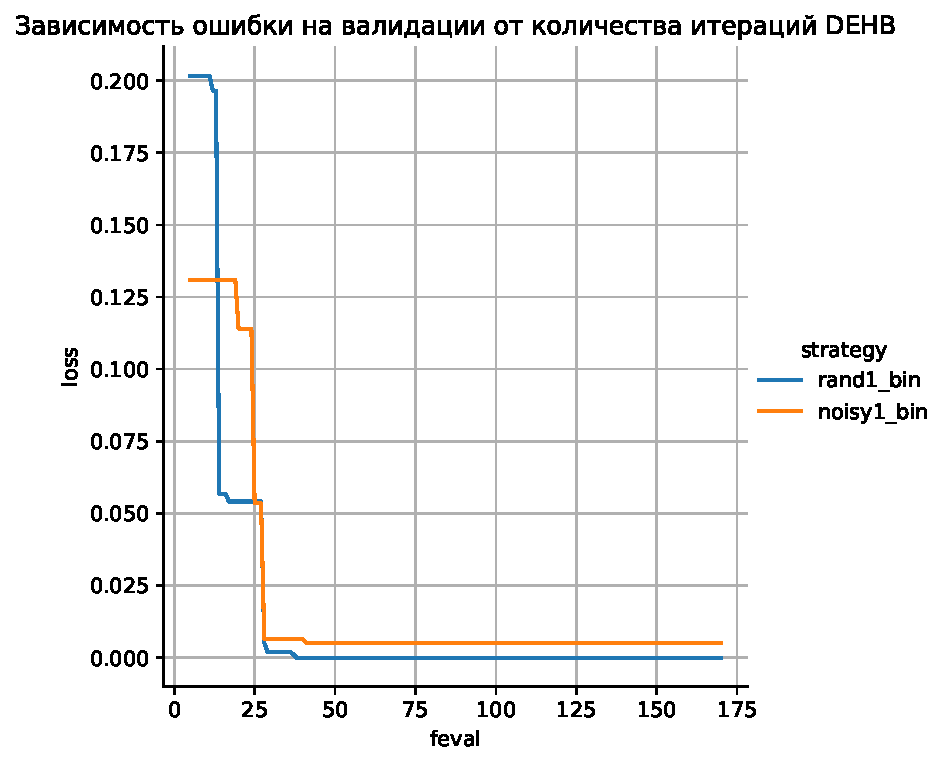
\includegraphics[width=7cm]{steel_plates_cmp.pdf}
%         &
%         \includegraphics[width=7cm]{liver_cmp.pdf} \\
%         Steel plates fault & Liver patients
%     \end{tabular}
%     \label{table:datasets1}
%     \caption{}
% \end{table}
\par

В задачах детекции брака стальных пластин и в задаче детекции пациентов с заболеваниями печени предложенный метод стабильно предсказывает лучшие наборы гиперпараметров, чем базовая стратегия мутации. Кроме того, даже несмотря на усреднение ошибок по различным запускам, невооруженным взглядом видно, что базовый метод без зашумления дольше выходит с каждого плато (``ступеньки'' на синем графике длиннее).

Сводная таблица итоговых ошибок и среднеквадратичных отклонений в методах:

\vspace{15px}

\makebox[\textwidth][c]{
\begin{tabular}{|l|l|l|l|l|l|}
\hline
Model/Data & 1                & 2                & 3                & 4               & 5                \\ \hline
DEHB           & $0.553\pm0.092$  & $0.001\pm0.005$  & $0.038\pm0.006$  & $0.242\pm0.012$ & $0.054\pm0.005$  \\ \hline
Proposed       & $0.542\pm0.081$* & $0.001\pm0.001$* & $0.035\pm0.006$* & $0.234\pm0.014$ & $0.051\pm0.005$* \\ \hline
\end{tabular}
}

\vspace{15px}

Видим, что предложенный метод показывает улучшение на большинстве датасетов.

\subsection{Анализ ошибки}
 
Используем датасет с данными о недвижимости для анализа зависимости ошибки метода от его гиперпараметров.
% \begin{table}[h]
%     \centering
%     \begin{tabular}{cc}
%         \includegraphics[width=7cm]{cali_housing_ablation.pdf}
%         &
%         \includegraphics[width=7cm]{cali_housing_step_ablation.pdf} \\
%         Зависимость от базового шума & Зависимость от величины шага
%     \end{tabular}
%     \label{table:datasets2}
%     \caption{}
% \end{table}
% \par
При рассмотрении зависимости от базового шума шаг равнялся 0. Видим, что на малом числе итераций нет значимой зависимости ошибки от параметров метода. Рассмотрим ошибку на наборе данных ilpd:

% \newpage

% \begin{table}[h]
%     \centering
%     \begin{tabular}{cc}
%         \includegraphics[width=7.3cm]{liver_ablation.pdf}
%         &
%         \includegraphics[width=7cm]{liver_step_ablation.pdf} \\
%         Зависимость от базового шума & Зависимость от величины шага
%     \end{tabular}
%     \label{table:datasets2}
%     \caption{}
% \end{table}
% \par
Видим, что явной монотонной зависимости от базового уровня шума нет. При этом на больших уровнях базового шума модель даже дольше находится на плато, так как новые конфигурации становятся слишком случайными и поиск идет в случайных областях вместо окрестности лучших наборов гиперпараметров.

При рассмотрении зависимости ошибки от величины шага видно, что слишком маленькие и слишком большие величины шага оказывают негативное влияние на ошибку на валидации. Однако видно, что при любых значениях метод позволяет выйти с плато и прийти к новым минимумам функции ошибок.

Также стоит заметить, что параметры метода стоит подбирать в зависимости от размерности пространства гиперпараметров, так как шум одной и той же величины с увеличением размерности будет вносить больший вклад в мутацию.

\section{Выводы}
Таким образом, предложенный метод показывает улучшение на некоторых датасетах. Добавление шума при выходе на плато позволяет получить новых кандидатов и продолжить подбор гиперпараметров с помощью дифференциальной эволюции.

Главной особенностью нового метода является гиперпараметр $m(t)$. Если взять его равным 0, то метод сводится к обычному DEHB. От выбора функции $m(t)$ зависит соотношение exploration/exploitation. При большим уровнях шума мутанты получаются полностью случайными, а при низких -- слишком близкими к кандидатам. Это одновременно является плюсом и минусом метода -- при удачно подобранном $m(t)$ алгоритм сможет быстро уходить с плато, а при неудачном -- покажет себя хуже классического DEHB.

Дальнейшими направлениями исследования являются изучение возможности добавления сэмплирования кандидатов из неисследованных участков пространства гиперпараметров, как это происходит в SMBO. Также можно изменить функции мутации -- например, сдвигать мутанта в направлении уменьшения значения функции ошибок. Функцию кроссовера также можно сделать более сложной -- не выбирать одно из двух значений, а брать промежуточное.

% \newpage

% \bibliographystyle{unsrtnat}
% \bibliography{references}

\end{document}